\section{Une propriété géométique de l'intégrale}

\begin{exercice}
    Soit $f$ de classe $\mathscr{C}^1$ sur $[a, b]$ telle que $f'$ soit strictement positive sur $[a, b]$. Calculer:
    $$\int_{a}^{b} f(t) \d t + \int_{f(a)}^{f(b)} f^{-1}(t) \d t.$$
\end{exercice}

\begin{elem_sol}
    \begin{enumerate}
    \item Comme $f' > 0$, alors $f$ est strictement croissante. Comme $f$ est continue, d'après le théorème de la bijection monotone, $f$ réalise une bijection de $[a, b]$ sur $[f(a), f(b)]$.
    
    \item On utilise le changement de variable $\phi : [a, b] \to [f(a), f(b)],\, u \mapsto f(u)$. Alors, $\phi$ est de classe $\mathscr{C}^1$ et
    \begin{align*}
    \int_{f(a)}^{f(b)} f^{-1}(t) \d t\\
    &= \int_a^b f^{-1}(f(u)) f'(u) \d u\\
    &= \int_a^b u f'(u) \d u\\
    &= \left[u f(u)\right]_a^b - \int_a^b f(u) \d u,
    \end{align*}
    où on a réalisé une intégration par parties.
    \end{enumerate}

    Finalement,
    \[
    \int_a^b f(t) \d t + \int_{f(a)}^{f(b)} f^{-1}(t) \d t = b f(b) - a f(a).
    \]
\end{elem_sol}



\todoinline{Une version plus claire de mon dessin ?}

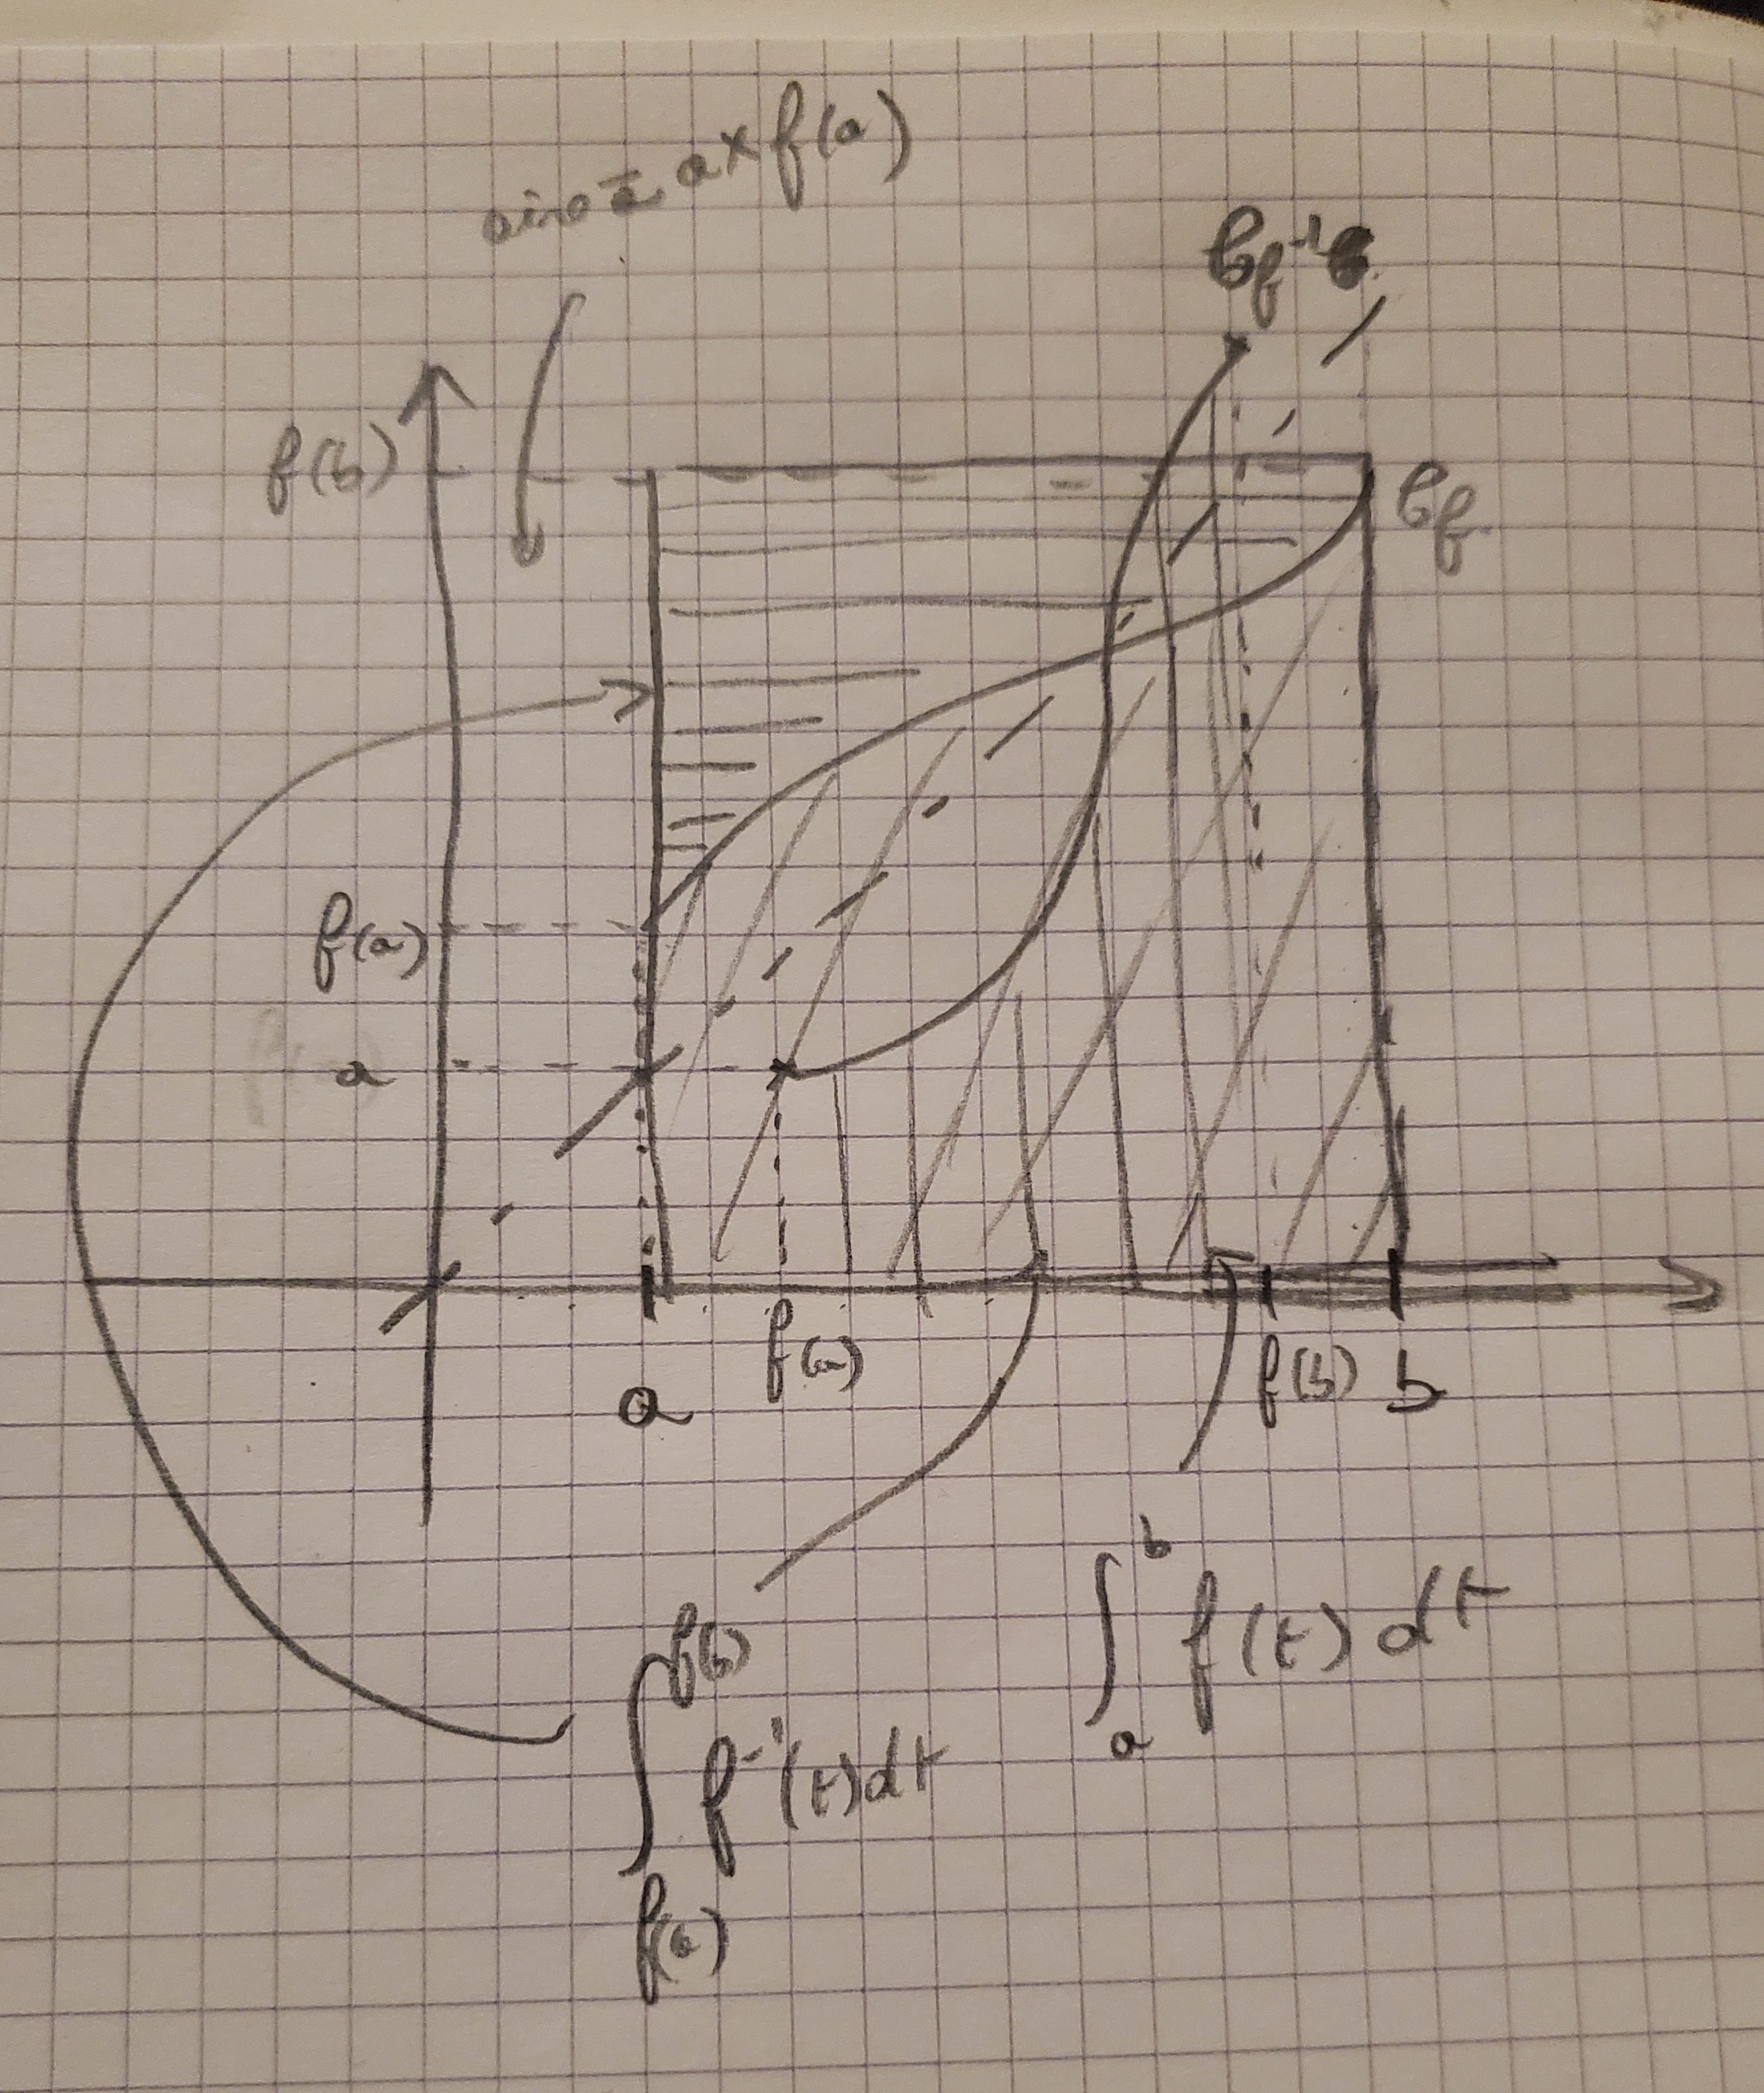
\includegraphics{./chapitres/integration/documents/propriete_geometrique.jpg}

Esquisse du dessin \\
\begin{tikzpicture}[line cap=round, >=latex]

    \def\x{0.5}
    \def\u{1.0}
    \def\v{0.3}
    \def\w{0.1}

    \draw[gray] (-.5, -.5) -- (5.5, 5.5) node[below left] {\contour{white}{\footnotesize$y = x$}};

    \path (1.5, 0.5)    coordinate (A)
        (2.5,2)    coordinate (B)
        (3.5, 5)  coordinate (C)
        (0.5, 1.5)    coordinate (A')
        (2,2.5)    coordinate (B')
        (5, 3.5)  coordinate (C');


    \begin{scope}
        \clip (A') ..controls +(0.5*\u, \u) and ( $(B') + (-\u, 0)$ )..
        (B') ..controls +(5*\v, 0) and ( $(C') + (-2*\v, -2*\v)$ )..
        (C') |- cycle;
        \foreach \x in {3.500,3.501,...,5.000}   
            \draw[blue!15!white, opacity=0.5] (\x,0) -- ++(0,10);
    \end{scope}
    
    \draw[thick, blue] 
        (A) ..controls +(\u, 0.5*\u) and ( $(B) + (0, -\u)$ )..
        (B) ..controls +(0, 5*\v) and ( $(C) + (-2*\v, -2*\v)$ )..
            (C) node[above] {$\mathcal{C}_{f^{-1}}$};
    \draw[thick, blue] 
        (A') ..controls +(0.5*\u, \u) and ( $(B') + (-\u, 0)$ )..
        (B') ..controls +(5*\v, 0) and ( $(C') + (-2*\v, -2*\v)$ )..
        (C') node[right] {$\mathcal{C}_f$};

    \fill[blue!15!white] (3.5,0) rectangle ++(1.5,1.5);
        
    \draw[dashed] (.5,0) node[black,below]{\footnotesize$a$} -- (A');
    \draw[dashed] (5,0) node[black,below]{\footnotesize$b$} -- (5,5);
    \draw[dashed] (1.5,0) node[black,below]{\footnotesize$f(a)$} -- (1.5,1.5);
    \draw[dashed] (3.5,0) node[black,below]{\footnotesize$f(b)$} -- (C);

    \draw[dashed] (0,.5) node[black,left]{\footnotesize$a$} -- (A);
    \draw[dashed] (0,5) node[black,left]{\footnotesize$b$} -- (5,5);
    \draw[dashed] (0,1.5) node[black,left]{\footnotesize$f(a)$} -- (1.5,1.5);
    \draw[dashed] (0,3.5) node[black,left]{\footnotesize$f(b)$} -- (C');

    \draw[->, black] (5.5,1.5) node[right] 
    {\footnotesize \contour{white}{$\displaystyle \int_a^b f(t)\, \mathrm{d} t$}} to [out=210,in=-20] ($(4.4,1.5)$);

    \draw (6.5,4) node[above] 
    {\footnotesize \contour{white}{$\displaystyle \int_{f(a)}^{f(b)} f^{-1}(t)\, \mathrm{d} t$}};

    \draw[thick, ->] (-.5, 0) -- (5.5, 0) node[above] {$x$};
    \draw[thick, ->] (0, -.5) -- (0, 5.5) node[left] {$y$};
    
\end{tikzpicture}